\documentclass[a4paper,11pt,titlepage]{jarticle}
\usepackage[dvipdfmx]{graphicx}
\usepackage{listings}
\usepackage{amsmath}
\usepackage{fancybox,ascmac}

\title{アルゴリズムとデータ構造 : 第一回レポート}
\author{175751C 宮城孝明}
\date{\today}

\begin{document}
\maketitle
\tableofcontents
\clearpage

\section{課題}
\lstinputlisting[language=C, numbers=left, breaklines=true, basicstyle=\ttfamily\footnotesize, frame=single, caption=課題プログラム, label=pg:algorithm]{algorithm.c}\par
こちらが実際の実行結果です\par
\begin{figure}[htbp]
  \centering
  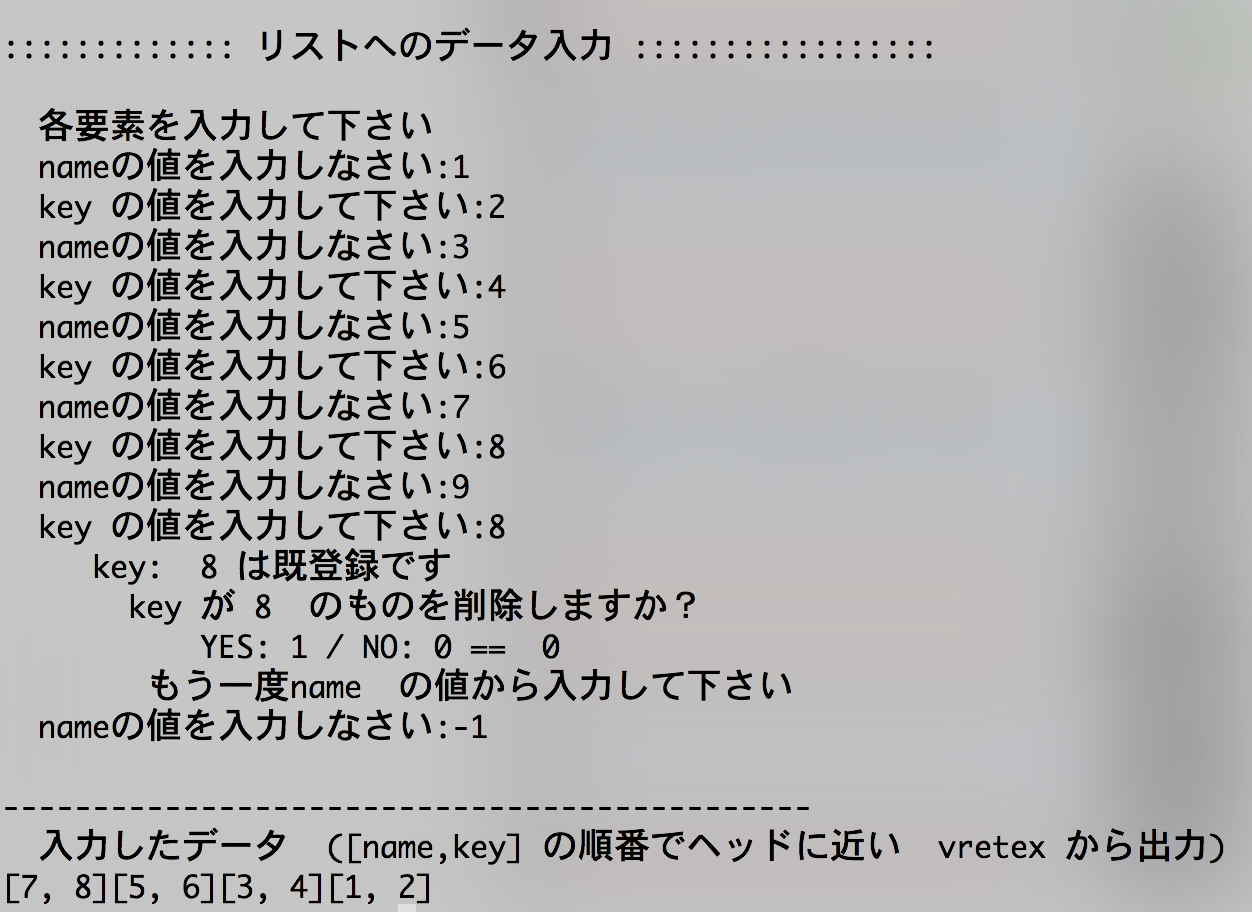
\includegraphics[width=100mm]{0523.png}
  \label{sample1}\\
\end{figure}

\begin{figure}[htbp]
  \centering
  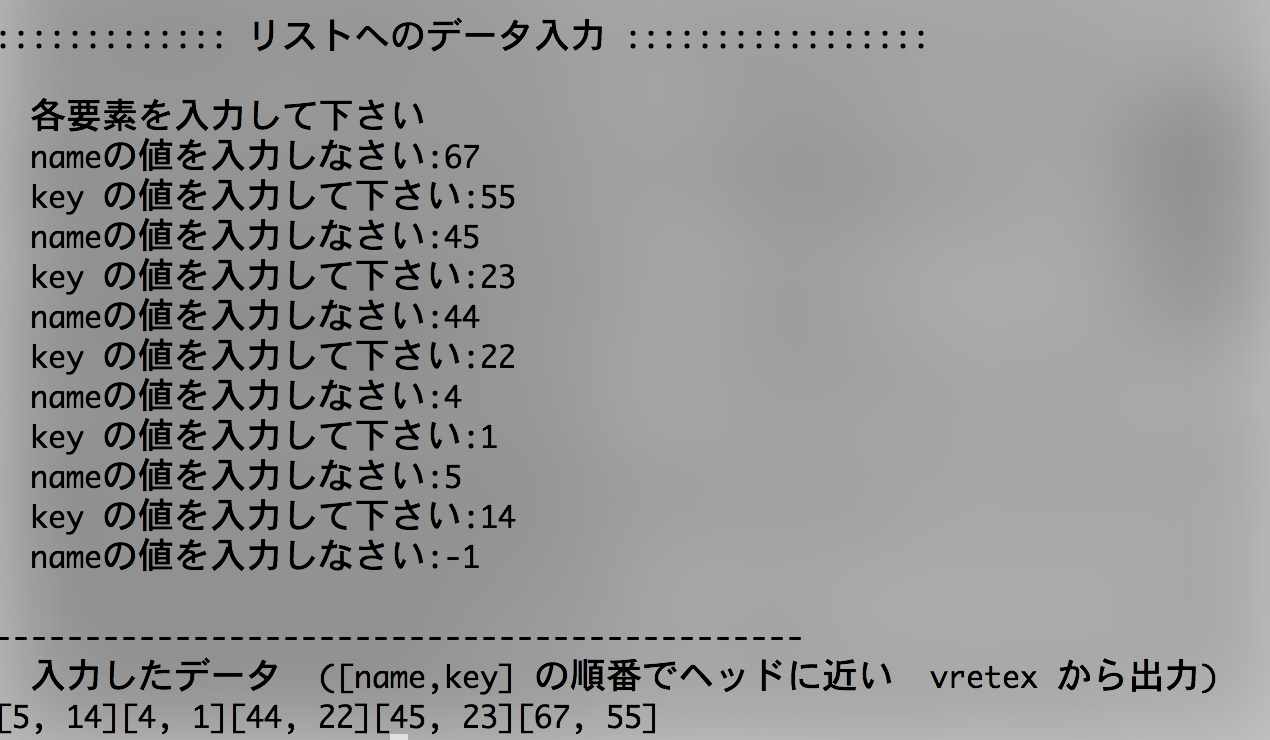
\includegraphics[width=100mm]{1357.png}
  \label{sample2}\\
\end{figure}

\begin{figure}[htbp]
  \centering
  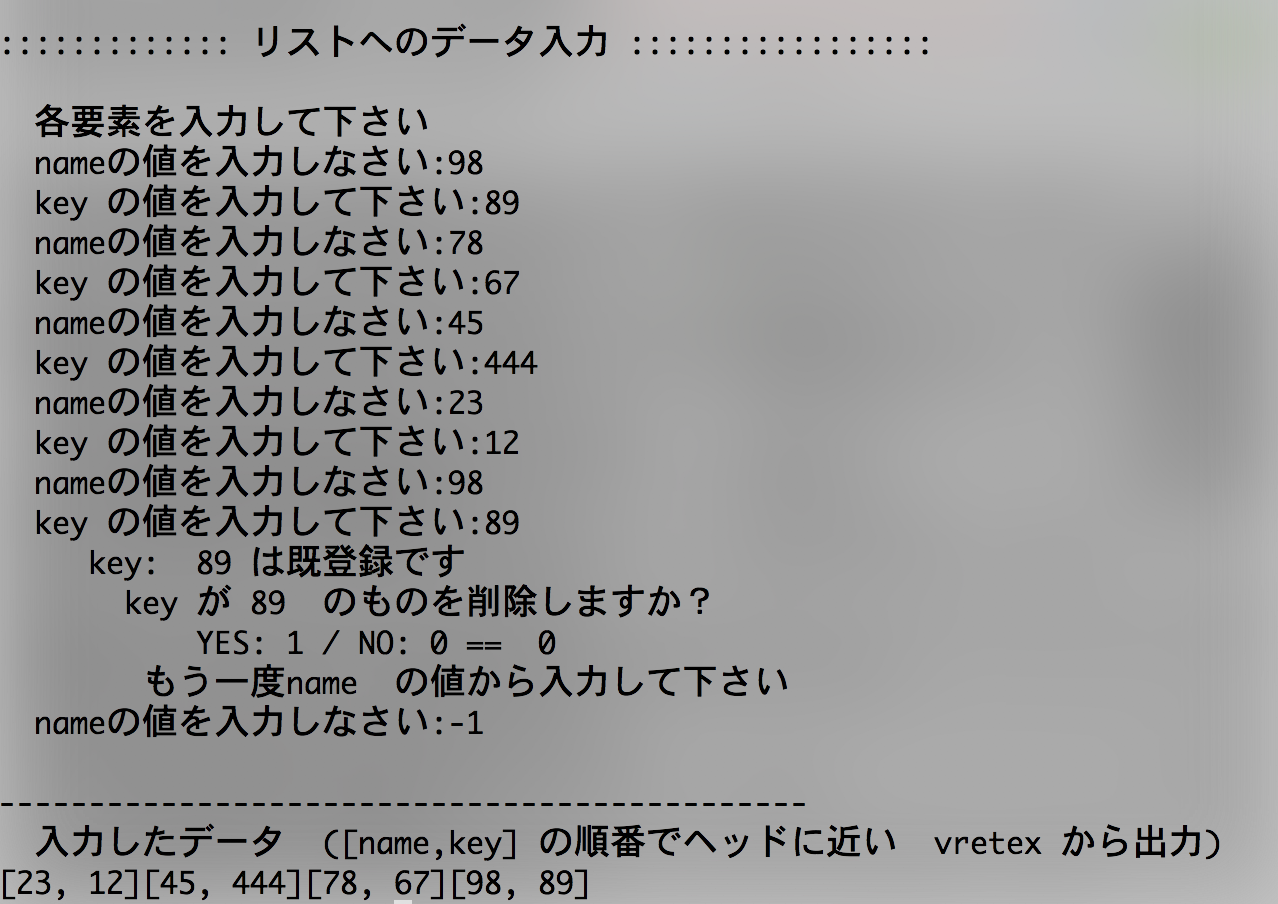
\includegraphics[width=100mm]{1358.png}
  \label{sample3}\\
\end{figure}

\begin{figure}[htbp]
  \centering
  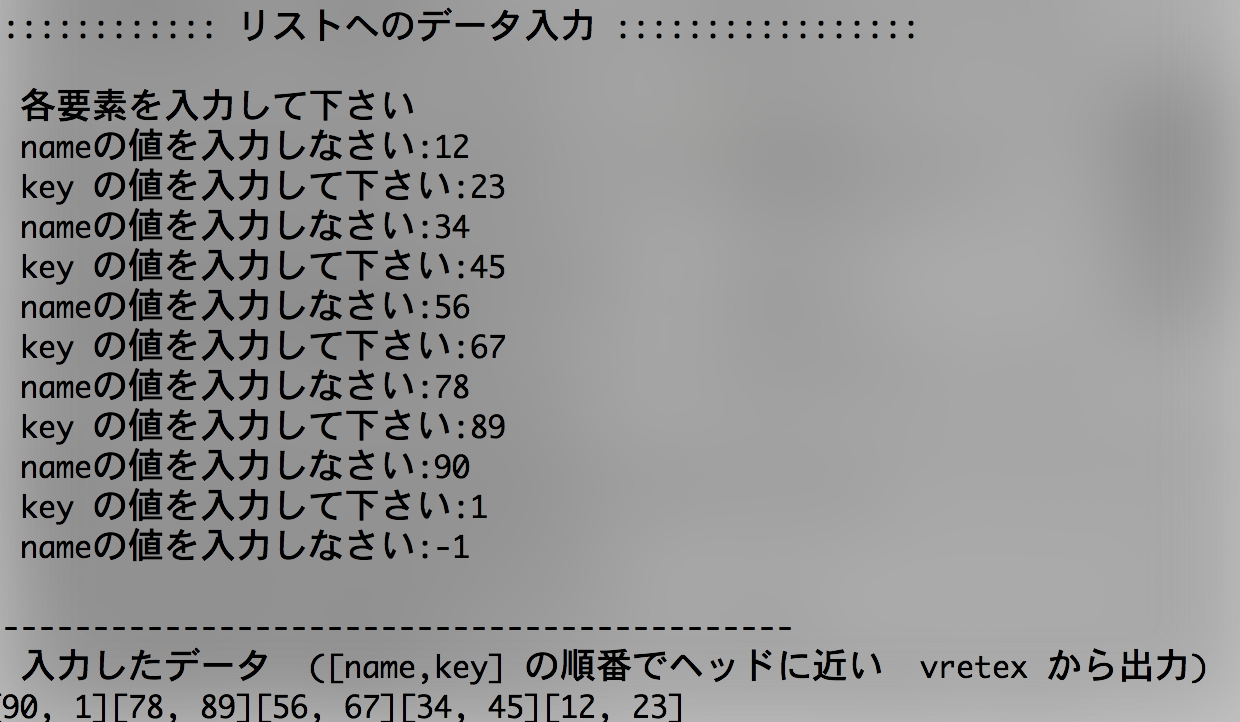
\includegraphics[width=100mm]{1359.png}
  \label{sample4}\\
\end{figure}\par
\par

これらの結果より、正しく実行していることがわかる。このプログラムは、nameとkeyにそれぞれ値を代入し、それをメモリに保存する。これをwhileの条件を満たしている間は、ずっと同じ入力の動作を実行してくれます。そして、nameに-1が代入されると、それまでに入力された数字をnameとkeyのくくりにして出力してくれます。


\end{document}
